\documentclass[10pt,a4paper,notitlepage]{article}
\usepackage[utf8]{inputenc}
\usepackage{amsmath}
\usepackage{amsfonts}
\usepackage{amssymb}
\usepackage{fullpage}
\usepackage{lastpage}
\usepackage{lscape}
\usepackage{fancyhdr}
\usepackage{multirow}
\usepackage{fancyvrb}
\usepackage{xcolor}
\usepackage{tikz}
\usepackage{graphicx}
\graphicspath{{./Graphics/}}
\usepackage{float}
\usepackage{nameref}
\usepackage[backend=bibtex,style=authortitle-ibid]{biblatex}
\addbibresource{References.bib}
  
\author{Jonah Gibbon}

\pagestyle{fancy}
\fancyhf{}
\renewcommand{\headrulewidth}{0pt}
\cfoot{Page \thepage\ of \pageref{LastPage}}

\newcommand{\abs}[1]{\lvert#1\rvert}
\newcommand{\Z}{\mathbb{Z}}
\newcommand{\Q}{\mathbb{Q}}
\newcommand{\C}{\mathbb{C}}
\newcommand{\N}{\mathbb{N}}
\newcommand{\R}{\mathbb{R}}
\newcommand{\Orb}{\text{Orb}}
\newcommand{\Id}{\text{Id}}
\newtheorem{theorem}{Theorem}


\renewcommand{\refname}{Reference}

\definecolor{brandeisblue}{rgb}{0.0, 0.44, 1.0}
\definecolor{bostonuniversityred}{rgb}{0.8, 0.0, 0.0}

\begin{document}
Throughout this project, permutations $\pi :X\rightarrow X$ will be represented in cyclic form, but also as $2\times n$ matrices (where the first row is the set $X$ and the second row is the corresponding image). For example the permutation $(1,2)(3,4)$ when $n=5$ could also be represented as
\begin{equation*}
\begin{pmatrix}
1&2&3&4&5\\
2&1&4&3&5
\end{pmatrix}
\end{equation*}
All code in this project will use the matrix representation, since permutations are represented uniquely this way.
\subsection*{\centering Question 1}
The program named \nameref{cd:1}, referenced on page \pageref{cd:1}, was used to multiply permutations together and calculate their inverses.\footnote{The functions \texttt{Multiply} and \texttt{Inverse} will now be used implicitly throughout the rest of the project. They will not be referenced in any further code.} The following permutations were used as test data.
\begin{equation*}
A=\begin{pmatrix}
1&2&3&4\\
3&4&2&1
\end{pmatrix} \quad\quad
B=\begin{pmatrix}
1&2&3&4\\
2&1&3&4\\
\end{pmatrix}
\end{equation*}
The code outputted the correct answers:
\begin{equation*}
AB=\begin{pmatrix}
1&2&3&4\\
4&3&2&1
\end{pmatrix}
\quad\quad
A^{-1}=\begin{pmatrix}
1&2&3&4\\
4&3&1&2
\end{pmatrix}
\end{equation*}
The program finds a permutation $\pi$'s inverse by calculating $\pi x$ for all $x\in X$, and saving $\pi^{-1}(\pi x)=x$. This exploits the fact that the permutation is a bijection; otherwise this method would fail. Calculating the image of an element requires $O(1)$ operations, and saving the appropriate value also requires $O(1)$ operations. We conclude that this method is $O(n)$.

When multiplying two permutations $\pi_{1}$ and $\pi_{2}$ together the method is similar. The program calculates $\pi_{1}x$, then $\pi_{2}(\pi_{1}x)$, and saves this as the image of $x$. This requires a total of $O(1)$ operations per element, and hence is $O(n)$ as well.

\subsection*{\centering Question 2}
We aim to prove by induction on $l$ that the set of permutations currently in the array, combined with the permutations $\pi_{l+1},\hdots,\pi_{k}$ generate $G$, where $\l$ is the number of generators added/omitted to array. Clearly this is true when $l=0$.

Suppose the case $l=m$ holds, where $m\in \N$. Also suppose that applying the algorithm to the permutation $\pi_{m+1}$ causes it to be modified $0\leq r\leq n$ times before either being discarded as the identity, or being added to the array. At this point, the permutation will be of the form $\pi'=g_{r}^{-1}g_{r-1}^{-1}\hdots g_{1}^{-1}g_{0}^{-1}\pi_{m+1}$, where each $g_{i}$ is some permutation currently in the array (with the exception $g_{0}$ being the identity). Should $\pi'$ be the identity, then $\pi_{m+1}$ can be generated from the current permutations in the array and so can be discarded from the generating set. If $\pi'$ is added to the array, then $\pi_{m+1}$ can still be generated from the current modified set, namely $\pi_{m+1}=g_{1}\hdots g_{r}\pi'$. Hence the inductive step holds. By setting $l=k$ the result follows immediately.\\

Notice that only the cells above the diagonal of the array ever gets filled. No permutation can get added on the diagonal, since then we would require the permutation to not fix some element in $X$, but also simultaneously fix that same element. If a permutation $\pi$ was added below the diagonal, say at position $(i,j)$ where $i>j$, then this permutation would not fix $i$, and in turn would not fix $j$ (since $i\mapsto j$). But then the algorithm would never have got to row $i$ in the first place, it would have stopped at (at least) row $j$, a contradiction. Therefore a bound for the total number of generators at the end of the algorithm is
\begin{equation}\label{eq:bound}
\min\left( k \, , \frac{n(n-1)}{2}\right)
\end{equation}
This proves that any subgroup of $S_{n}$ can be generated by at most $n(n-1)/2$ elements.\\

This leads to the natural question - what is the minimum number of generators needed to produce any subgroup of $S_{n}$? We can find the better bound of only $n-1$ generators, by first decomposing $G$ into a strong generating set (something that will be focus of Question 8). Essentially, we may find subgroups $G_{i}$ which stabilise elements $\alpha_{1},\hdots,\alpha_{i}$, and $G=G_{0}\geq G_{1}\geq\hdots \geq G_{r}=1$, where each inclusion is strict. Starting with $G_{r}$ we recursively add generators until we produce $G$, where each generator decreases the number of different orbits when the current subgroup acts on $G$. Since $G_{r}$ gives $n$ different orbits (it fixes every element in $G$), the number of generators for $G$ can be bounded by $n-t$, where $t$ is the number of different orbits in $G$, and since $t\geq 1$ the result follows.\footnote{A more rigorous proof is presented in \cite{JERRUM198660}}\\

To bound the number of operations of the stripping algorithm, we first look at how to process one permutation $\pi$. On the $i$th row of the array,  the algorithm will check if $\pi(i)=i$ ($O(1)$ operation), as well as check if the $\pi(i)$th cell is empty ($O(1)$ operation). Based on the outcome, the algorithm will either save the permutation ($O(n)$ operations), modify it ($O(n)$ operations from Question 1) or move directly onto row $i+1$. The worst of these options is if the permutation is modified, since it has the largest complexity, and the code cannot immediately move onto the next permutation. Assuming the longest running time, a permutation will be modified on all $n$ rows before being discarded,  taking $O(n^{2})$ in total. Therefore an upper bound for the number of operations for this algorithm is $O(kn^{2})$.

\subsection*{\centering Question 3}
\nameref{cd:3}, referenced on page \pageref{cd:3}, implements the Stripping Algorithm of Sims.\footnote{The function \texttt{SAOS} defined in \nameref{cd:3} will be used implicitly throughout the rest of the project. It will no longer be referenced in any further code.} The following input was used to test if the code was working properly:
\begin{equation*}
\pi_{1}=(1,2) \quad\quad \pi_{2}=(1,2,3) \quad\quad \pi_{3}=(2,3,5) \quad\quad \pi_{4}=(1,5,3) \quad\quad \pi_{5}=\Id \quad\quad n=5
\end{equation*}
The group generated is equal to $S_{4}$ (up to relabelling), since we can produce consecutive transpositions $(2,3)=\pi_{1}\pi_{2}$ and $(3,5)=\pi_{1}\pi_{2}\pi_{3}$, and all generators fix the element 4. The output given was the set of permutations 
\begin{equation*}
\pi_{1}'= (1,2) \quad\quad \pi_{2}'=(2,3) \quad\quad \pi_{3}'=(3,5) \quad\quad \pi_{4}'=(1,5,3)
\end{equation*}
confirming the results of Question 2. Notice that the number of generators outputted are less than $k=5$ and $n(n-1)/2=10$, confirming the result in equation \eqref{eq:bound}. However it hasn't reduced the number of generators completely, since $\pi_{4}'$ is redundant and can be generated from the first three (equals $\pi_{3}'\pi_{2}'\pi_{1}'\pi_{2}'$). This method serves as an efficient way to keep the number of generators of a permutation group relatively small, but will not output the smallest set of generators.\\

\subsection*{\centering Question 4}
Define the map $f: \Orb_{G}(\alpha) \rightarrow \lbrace \text{left cosets of } G_{\alpha}\rbrace$ by sending $g(\alpha) \mapsto gG_{\alpha}$. We first check that this map is well defined; if $g\left(\alpha\right)=h\left(\alpha\right)$ then $gG_{\alpha}=hG_{\alpha}$. We know $h^{-1}g(\alpha)=\alpha$ so $h^{-1}g\in G_{\alpha}$, or $gG_{\alpha}=hG_{\alpha}$. This map is injective, since if $gG_{\alpha}=hG_{\alpha}$ then $h^{-1}g\in G_{\alpha}$. So $h^{-1}g(\alpha)=\alpha$ or $h(\alpha)=g(\alpha)$. The map is also surjective, since all left cosets $gG_{\alpha}$ have the corresponding $g(\alpha)$ in $\Orb_{G}\left(\alpha\right)$ by the definition of an orbit. Therefore this map is a bijection. \\

The Orbit-Stabiliser theorem is as follows: Let $G$ be a finite group acting on a set $X$. Then for all $\alpha\in X$, $\abs{G}=\abs{\Orb_{G}\left(\alpha\right)} \cdot \abs{G_{\alpha}}$. The proof uses the fact that the set of left cosets of $G_{\alpha}$ partitions $G$,\footnote{A proof of this is covered in Part 1A Groups.} and therefore $\abs{\lbrace \text{left cosets of }G_{\alpha}\rbrace}\cdot \abs{G_{\alpha}}=\abs{G}$. Using the bijection in the first part, $\abs{\Orb_{G}\left(\alpha\right)}=\abs{\lbrace \text{left cosets of } G_{\alpha}\rbrace}$, and the result follows. 

\subsection*{\centering Question 5}
\nameref{cd:5}, referenced on page \pageref{cd:5}, was used to calculate the orbit of an element $\alpha\in X$.\footnote{The function \texttt{Orbit} defined in Code 5 will be used implicitly throughout the rest of the project, and will no longer be included in subsequent referencing.} The following test data was used: $\pi_{1}=(2,3,4)$, $\pi_{2}=(1,5)$, $\alpha=2$, $n=5$, and the correct output was
\begin{table}[H]
\centering
\begin{tabular}{|c|c|}
\hline Image of $\alpha=2$ & Witness Permutation \\
\hline 2 & $\Id$\\
3 & $(2,3,4)$\\
4 & $(2,4,3)$\\
\hline
\end{tabular}
\caption{Test data for Question 5}
\end{table}
To calculate the orbit of $\alpha$, the code starts by creating a 'queue' which initially only contains $\alpha$. It also creates a $n\times 2$ array which will save the elements of the orbit with their corresponding witnesses, and will also act as a hash table for efficient indexing. It proceeds to apply each generator to the first element in the queue, and saves any new element $i$ to the $i$-th row of the array, as well as the generator that created it. It then adds $i$ to the back of the queue. The code iterates through the elements of this queue, applying each generator to the current element,  saving any new elements $i$ and the generators that produced them, and appending these $i$ to the back of the queue. The code will terminate when we reach the end of this queue.\\

This method does indeed produce the complete orbit. Suppose $\beta \in \Orb_{G}(\alpha)$, then $\beta = \pi_{r}\hdots \pi_{1} (\alpha)$ where each $\pi_{i}$ is a generator, and $r$ is the smallest integer where this is possible. Let $P_{i}=\pi_{i}\hdots\pi_{1}(\alpha)$, so that $P_{r}=\beta$. Then each $P_{i}$ must be unique, otherwise we could find a smaller value for $r$. Therefore, by only testing new elements in the queue, we will generate the entire orbit. \\

The complexity of the algorithm is bounded by $O(kn^{2})$, where $k$ is the number of generators of $G$. For each element in the queue, $k$ generators are applied to it, each taking $O(1)$ operations. It checks if any new element has been produced, which is why the additional array was created - it allows the code to check if element $i$ has already been produced with complexity $O(1)$ (not searching $O(n)$) since $i$ would be saved in position $i$. However this does mean this code requires more memory to run. If this element has not been produced, it will save the element, and permutation that produced it, which is $O(n)$. Therefore for each element in the queue, the complexity is bounded by $O(kn)$, and since the queue has length at most $n$, the total complexity is bounded by $O(kn^{2})$.

\subsection*{\centering Question 6}
We aim to prove by induction that $t_{i+1}=\varphi(y_{i}\hdots y_{1})$. If $g=hz$, where $g, h\in G$ and $z\in G_{\alpha}$,  then $gG_{\alpha}=hzG_{\alpha}=hG_{\alpha}$ and so $\varphi(g)=\varphi(h)$. When $i=1$, $t_{2}=\varphi(y_{1}t_{1})$, but $t_{1}\in G_{\alpha}$ and so $t_{2}=\varphi(y_{1})$ and the base case holds. Now assume that $t_{k+1}=\varphi(y_{k}\hdots y_{1})$ for some $k\in \Z$. We know that $y_{k}\hdots y_{1}=\varphi(y_{k}\hdots y_{1}) g$ for some $g\in G_{\alpha}$ (left cosets partition $G$), so $t_{k+2}=\varphi(y_{k+1}\varphi(y_{k}\hdots y_{1}))=\varphi(y_{k+1}y_{k}\hdots y_{1}g^{-1})$. But $g^{-1}\in G_{\alpha}$, so this equals $\varphi(y_{k+1}\hdots y_{1})$. Therefore the inductive step holds. Immediately we conclude $t_{r+1}=\varphi(y_{r}\hdots y_{1})=\varphi(x)=t_{1}$.\\

Let $S=\langle \lbrace \varphi(yt)^{-1}\cdot y\cdot t \,\,\vline \, \, y\in Y, t \in T\rbrace\rangle$ and $t_{1}=t_{r+1}=1$; the identity. Then
\begin{equation*}
\begin{aligned}
x &= t_{r+1}^{-1}\cdot y_{r}\cdot t_{r}\cdot t_{r}^{-1}\cdot y_{r-1}\cdot t_{r-1} \cdot t_{r-1}^{-1} \cdot y_{r-2} \cdot t_{r-2} \hdots t_{2}^{-1}\cdot y_{1}\cdot t_{1}\\
&=\varphi(y_{r}t_{r})^{-1}y_{r}t_{r}\cdot \varphi(y_{r-1}t_{r-1})^{-1}y_{r-1}t_{r-1}\hdots \varphi(y_{1}t_{1})y_{1}t_{1}
\end{aligned}
\end{equation*}
It is visible that $x$ can be generated by the elements in $S$,  and since $x$ was arbitrary, $G_{\alpha}\leq S$. To check the other inclusion, notice that $yt=\varphi(yt)g$, for some $g\in G_{\alpha}$, and so $yt(\alpha)=\varphi(yt)(\alpha)$. Therefore $\varphi(yt)^{-1}yt(\alpha)=\alpha$, and so all the generators fix $\alpha$. Therefore $G_{\alpha}\geq S$, and so conclude that $G_{\alpha}=S$.\\

\subsection*{\centering Question 7}
\nameref{cd:7}, referenced on page \pageref{cd:7}, was used to produce a generating set for the stabiliser of an element.\footnote{The function \texttt{Stabiliser} defined in Code 7 will be used implicitly throughout the rest of the project, and will not be included in subsequent referencing.} It works as follows: since the orbits form a bijection with the set of left cosets of $G_{\alpha}$, the permutations produced by Code 5 form a complete set for $T$.  Since each of these permutations send $\alpha$ to a different element, we use this to define the $\varphi$ function. The code then iterates through creating $S$, and reduces it with the stripping algorithm. \\

The following test data was used: $Y=\lbrace (1 \, 2), (1 \, 2 \, 3 \, 4 \, 5)\rbrace$, $n=5$ and $\alpha=5$. In Question 9 there is a proof that $\langle Y \rangle=S_{5}$, and so we expect the stabiliser to equal to $S_{4}$, made up of all permutations that fix 5. The output was the set of generators 
\begin{table}[H]
\centering
\begin{tabular}{|c|}
\hline Stabiliser for $\alpha=5$ \\
\hline $(1,2)$\\
$(1,3)$\\
$(1,4)$\\
$(2,3,4)$\\
\hline
\end{tabular}
\caption{Test data for Question 7}
\end{table}
The first three of these generate $S_{4}$, confirming this code works. \\
Question 5 already has complexity $O(kn^{2})$.  Since $\abs{Y}=k$ and $\abs{T}\leq n$, then the set that generates $G_{\alpha}$ will have size at most $kn$. Each permutation has to be stored, taking a total of $O(kn^{2})$ operations. Finally applying the stripping algorithm to the set of $kn$ generators gives $O(kn^{3})$ operations. Therefore computing the generators of a stabiliser is bounded by $O(kn^{3})$.

\subsection*{\centering Question 8}
By producing a stabiliser chain $G=G_{0}\geq G_{1}\geq G_{2}\geq \hdots \geq G_{r}=\lbrace e\rbrace$, where $G_{i}$ is the stabiliser for elements $\alpha_{1},\hdots,\alpha_{i}$, each of which have been picked such that $\abs{\Orb_{G_{i-1}}(\alpha_{i})}> 1$, we can conclude from repeatedly applying the Orbit Stabiliser theorem that
\begin{equation}
\abs{G}=\prod_{i=1}^{r}\abs{\Orb_{G_{i-1}}(\alpha_{i})}
\end{equation}
Notice $\abs{G}\leq \abs{S_{n}}=n!$ is finite, so the orbit stabilizer theorem applies. \\

This is an efficient way of calculating the size of a permutation group. Suppose there were $k$ initial generators, so stripping them would take $O(kn^{2})$ operations and give a generating set of size less than $n^{2}$ (from equation \eqref{eq:bound}). Iterating through $X$ to find an element $\alpha_{i}$ with a non-trivial orbit would therefore take at most $O(n^{2}\cdot n^{2}\cdot n)$ operations. Calculating the corresponding stabilizer (from Question 7) would also take $O(n^{2}\cdot n^{3})$ operations, with this stabilizer having at most $n^{2}$ generators as well. All of this would iterate at most $\log_{2}\left(\abs{G}\right)$ times, and so we conclude that the algorithm has complexity at most.
\begin{equation}
O\left(\log_{2}\left(\abs{G}\right)n^{5}\right)
\end{equation}
Since $\abs{G}\leq n!\leq n^{n}$, $\log_{2}\left(\abs{G}\right)\leq n^{2}$. Hence this algorithm runs in polynomial time.\\

If we didn't use the stripping algorithm at every stage, the number of generators would grow out of control. Suppose $k$ generators were initially inputted in Code 8,  and $G_{i}$ and $\alpha_{i}$ are defined as in the start of this question. Then after the first iteration we would have saved $k\times\abs{T}=k\times \abs{\Orb_{G_{0}}(\alpha_{1})}$ generators, after the second iteration we would have saved $k\times \abs{\Orb_{G_{0}}(\alpha_{1})}\times \abs{\Orb_{G_{1}}(\alpha_{2})}$, and after the code had completed we would have saved $k\abs{G}$ generators. A lower bound for the complexity would therefore be $O(kn\abs{G})$, since each generator would have to be saved. Should $\abs{G}$ be large ($20!\approx 10^{18}$) a large amount of memory would be required. More importantly, since $\abs{G}$ could equal $n!$ then this program would run in exponential time, and so is not efficient.\\

Code 8, referenced on page \pageref{cd:8}, was used to calculate the order of the group produced by a set of given generators.\footnote{The function \texttt{Order} defined in \nameref{cd:8} will no longer be included in subsequent referencing.} The following set was used as test data:
\begin{equation*}
y_{1}=(1,2,3) \quad \quad y_{2}=(1,2,4)  \quad \quad y_{3}=(1,2,5)  \quad \quad y_{4}=(1,2,6)  \quad \quad n=6
\end{equation*}
The output was the table
\begin{table}[H]
\centering
\begin{tabular}{c|c|c|c|c|c}
$i$ & $\abs{G_{i}}$ & Gens before strip & Gens after strip & $\alpha_{i+1}$ & $\abs{\Orb_{G_{i}}(\alpha_{i+1})}$\\
\hline 0& 360 & 4 & 4 & 1 & 6\\ 
1& 60 & 24 & 9 & 2 & 5\\ 
2& 12 & 45 & 5 & 3 & 4\\ 
3 & 3 & 20 & 2 & 4 & 3\\
4 & 1 & 6 & 0 & $\ast$ & $\ast$ \\

\end{tabular}
\caption{Test data for Code 8}
\end{table}
Therefore $\abs{G}=360$. This means that $G=A_{6}$, since the generators only contain even permutations and $6!/2$ different permutations have been produced.\footnote{It is true in general that $A_{n}$ is generated by the permutations $(1,2,3),\hdots ,(1,2,n)$. A proof is laid out in Theorem 3.3 in \cite{PermStuff}.}\\

Another application of this code is to calculate the number of Rubik's Cube combinations. Each configuration can be represented as a permutation of 48 elements, more exactly, these are the 48 'outer' parts of each face. The figure below represents an example of such a numbering.

\begin{figure}[H]
\centering
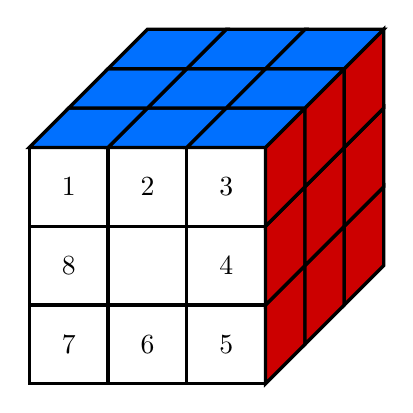
\begin{tikzpicture}[very thick]
\draw (0,0) rectangle (1,1);
\draw (1,0) rectangle (2,1);
\draw (2,0) rectangle (3,1);
\draw (0,1) rectangle (1,2);
\draw (1,1) rectangle (2,2);
\draw (2,1) rectangle (3,2);
\draw (0,2) rectangle (1,3);
\draw (1,2) rectangle (2,3);
\draw (2,2) rectangle (3,3);
\draw[yslant=1,xshift=3cm,yshift=-3cm,fill=bostonuniversityred] (0,0) rectangle (0.5,1);
\draw[yslant=1,xshift=3cm,yshift=-2cm,fill=bostonuniversityred] (0,0) rectangle (0.5,1);
\draw[yslant=1,xshift=3cm,yshift=-1cm,fill=bostonuniversityred] (0,0) rectangle (0.5,1);
\draw[yslant=1,xshift=3.5cm,yshift=-3cm,fill=bostonuniversityred] (0,0) rectangle (0.5,1);
\draw[yslant=1,xshift=3.5cm,yshift=-2cm,fill=bostonuniversityred] (0,0) rectangle (0.5,1);
\draw[yslant=1,xshift=3.5cm,yshift=-1cm,fill=bostonuniversityred] (0,0) rectangle (0.5,1);
\draw[yslant=1,xshift=4cm,yshift=-3cm,fill=bostonuniversityred] (0,0) rectangle (0.5,1);
\draw[yslant=1,xshift=4cm,yshift=-2cm,fill=bostonuniversityred] (0,0) rectangle (0.5,1);
\draw[yslant=1,xshift=4cm,yshift=-1cm,fill=bostonuniversityred] (0,0) rectangle (0.5,1);
\draw[xslant=1,yshift=3cm,xshift=-1cm,fill=brandeisblue](0,0) rectangle (1,0.5);
\draw[xslant=1,yshift=3cm,xshift=-2cm,fill=brandeisblue](0,0) rectangle (1,0.5);
\draw[xslant=1,yshift=3cm,xshift=-3cm,fill=brandeisblue](0,0) rectangle (1,0.5);
\draw[xslant=1,yshift=3.5cm,xshift=-1cm,fill=brandeisblue](0,0) rectangle (1,0.5);
\draw[xslant=1,yshift=3.5cm,xshift=-2cm,fill=brandeisblue](0,0) rectangle (1,0.5);
\draw[xslant=1,yshift=3.5cm,xshift=-3cm,fill=brandeisblue](0,0) rectangle (1,0.5);
\draw[xslant=1,yshift=4cm,xshift=-1cm,fill=brandeisblue](0,0) rectangle (1,0.5);
\draw[xslant=1,yshift=4cm,xshift=-2cm,fill=brandeisblue](0,0) rectangle (1,0.5);
\draw[xslant=1,yshift=4cm,xshift=-3cm,fill=brandeisblue](0,0) rectangle (1,0.5);
\node (1) at (0.5,2.5) {1};
\node (2) at (1.5,2.5){2};
\node (3) at (2.5,2.5){3};
\node (4) at (2.5,1.5){4};
\node (5) at (2.5,0.5){5};
\node (6) at (1.5,0.5){6};
\node (7) at (0.5,0.5){7};
\node (8) at (0.5,1.5){8};
\end{tikzpicture}
\caption{Rubik's Cube with the white face labelled}
\end{figure}

The generators of this group are the 90 degree rotations of each face, referenced on page \pageref{perms} as tables. The answer is the surprising large number 
\begin{equation*}
\abs{G}=43252003274489856000
\end{equation*}
This is testament to the method behind this algorithm, that it would be near impossible to list all combinations, but the algorithm works in $O\left(\log_{2}\left(\abs{G}\right)n^{5}\right)\approx O(10^{10})$ operations, a program most commercial computers could implement.

A major application of this algorithm which does not appear immediately obvious is that we can efficiently test an element for membership in finite groups. Given a set of generators $\pi_{1},\hdots,\pi_{k}$ for a known group $G$, we calculate the size of the group generated by the new set $\pi_{1},\hdots,\pi_{k}, x$ for some element $x$.  Should this be equal to $\abs{G}$, then we conclude that $x$ must lie in this group. Otherwise, we can conclude that it doesn't. 

An example of this is the Rubik's subgroup generated by 5 face rotations instead of 6. By adding the 6th rotation, the size of the group does not increase, proving that there exists \textit{some} combination of the 5 face rotations that produces the 6th.

By outputting the order of a group, a lot can be determined about its structure. This method could give a way of determining if certain permutation groups are not simple by applying the Sylow theorems. These theorems depend on the prime factorisation of the size of a group (currently a difficult task that cannot be done in polynomial time), however this algorithm already gives the answer in a partially factorised form, allowing for quicker processing.

\subsection*{\centering Question 9}
The two permutations $(1,2)$ and $(1,2,\hdots,n)$ generate $S_{n}$. Let $\sigma=(1,2,\hdots,n)$. Then 
\begin{equation}
\sigma^{k}(1,2)\sigma^{-k}=(\sigma^{k}(1),\sigma^{k}(2))=(k+1,k+2)
\end{equation}
But consecutive transpositions generate $S_{n}$ and hence the set $\lbrace (g,h)\in S_{n}\times S_{n} : \langle g,h\rangle =S_{n}\rbrace$ is non-empty and $P_{n}>0$.\footnote{A straightforward proof that consecutive transpositions generate $S_{n}$ is laid out in \cite{PermStuff}}

If $(g,h)\in A_{n}\times A_{n}$ then no odd permutation could be produced by these generators. Since $\abs{A_{n}}=n!/2$, the probability that this occurs is $1/4$, and therefore $P_{n}\leq 3/4$ ($k=3/4$). This is only true for $n\geq 2$, since $A_{1}=S_{1}=\lbrace 1\rbrace$. \\

When $n$ is very small we can calculate each of the combinations of permutations, and by brute force find $P_{n}$. However there are $n!(n!-1)/2$ combinations to check, which diverges quickly, and so this method is not feasible for large $n$. \nameref{cd:9.1}, referenced on page \pageref{cd:9.1}, was used to calculate the exact values of $P_{n}$ for $1\leq n\leq 6$. 
\begin{table}[H]
\centering
\begin{tabular}{|c|c|}
\hline $n$ & $P_{n}$ \\
\hline 1 & 1\\
2 & 3/4\\
3 & 1/2\\
4 & 3/8\\
5 & 19/40\\
6 & 53/120\\
\hline
\end{tabular}
\caption{Exact values for $P_{n}$}\label{tb:Exact P_n}
\end{table}

We can see that the values aren't larger than 3/4, apart from the case when $n=1$, as discussed. \\

To generate a random permutation we could pick a random number from a list from 1 to $n$, save this as the image of 1. Then pick a random element from this list, and if it hasn't already been chosen, set this as the image of 2, and so on. However this is inefficient, since it unnecessarily checks to see if numbers have already been chosen. Instead we can generate permutations using the Fisher-Yates shuffling algorithm, which does not require these checks. It starts with an arbitrary permutation, say the identity, and chooses a random number $\gamma_{1}$ from 1 to $n$. It then proceeds to switch the $n$-th element with the $\gamma_{1}$-th element. It then generates a random number $\gamma_{2}$ from 1 to $n-1$, and switches element $n-1$ with $\gamma_{2}$, and so forth. A simple induction proves that this method is unbiased, and we can see that this does not require to check that any element has already been taken. 

Suppose we wish to estimate $P_{n}$ for $1\leq n\leq k$ for some $k\in \Z$, accurate to 2 decimal places at a $0.95$ confidence level. We would therefore have to estimate a single $P_{n}$ at a $\sqrt[k]{0.95}$ confidence level. Suppose $m$ independent samples $X_{i}\sim\text{Bernoulli}(P_{n})$ are taken. If $m$ is sufficiently large, by the central limit theorem we can assume 
\begin{equation}
\frac{1}{m}\sum_{i=1}^{m}X_{i}\sim P_{n}+\frac{\sqrt{P_{n}\left(1-P_{n}\right)}}{\sqrt{m}}Y
\end{equation}
where $Y\sim \mathcal{N}(0,1)$. Therefore a $\sqrt[k]{0.95}$ confidence interval is $[-\Phi((1+\sqrt[k]{0.95})/2),\Phi((1+\sqrt[k]{0.95})/2)]$. Maximising $\sqrt{P_{n}(1-P_{n})}$ over $P_{n}\in[0,1]$ gives 1/2, and so it suffices to choose a sample of size
\begin{equation}
m=\left(\Phi\left(\frac{1+\sqrt[k]{0.95}}{2}\right)\times 10^{2}\right)^{2}
\end{equation}
When $k=14$, $m\approx 8.4\times 10^{4}$, which is too large. However choosing $846<m$ ensures all estimates should be accurate to at least one decimal place, to give an indication of accuracy.\\

\nameref{cd:9.2}, referenced on page \pageref{cd:9.2}, was used to generate random permutations and produce estimates for $P_{n}$ when $k=14$, as well as plot them against $n$ in Figure \ref{fg:P_n estimates}, when $m=3000$.
\begin{figure}[H]
\centering
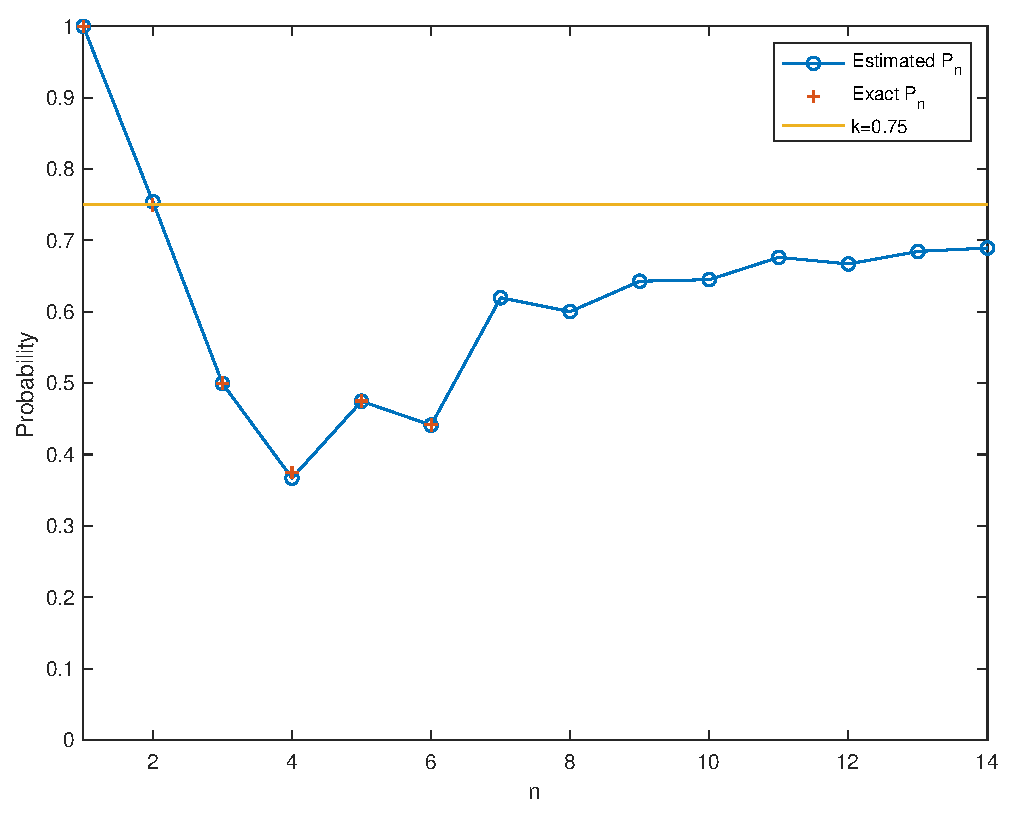
\includegraphics[width=12cm]{Image_1}
\caption{$P_{n}$ for different $n$}\label{fg:P_n estimates}
\end{figure}
Firstly we see that the first few estimates are incredibly close to the exact values of $P_{n}$ in Table \ref{tb:Exact P_n}, which confirms the algorithm is indeed producing random permutations. We can also see that $0<P_{n}\leq 3/4$, confirming the argument at the start of the question. 

An interesting feature is that it appears that $P_{n}$ tends to some constant. This is in fact true, with $P_{n}\rightarrow 3/4$ as $n\rightarrow \infty$. This is a corollary on Dixen's theorem, which states the proportion of pairs of permutations from $S_{n}$ that generate either the group $S_{n}$ or $A_{n}$ is greater than
\begin{equation}
1-\frac{2}{\left(\log\log n\right)^{2}}
\end{equation}
for sufficiently large $n$.\footnote{The proof that Dixen presented can be found in \cite{DIXEN}} We can see that this lower bound tends to 1, and since the probability that at least one of the generators being odd is 3/4, the result follows.

\section*{\centering References}\label{References}
\printbibliography[heading=none]

\pagebreak
\subsection*{\centering Rubik's Cube Permutations}\label{perms}
These are the generators inputted into \nameref{cd:8} when calculating the size of the Rubik's Cube group. A $2 \times 48$ size table won't fit onto this document, so only the elements that get changed by the generator have been noted, and all other faces on the Rubik's Cube that have been omitted can be considered fixed.
\begin{table}[H]
\centering
\begin{tabular}{|cccccccccccccccccccc|} \hline
1 & 2 & 3 & 4 & 5 & 6 & 7 & 8 & 9 & 15 & 16 & 27 & 28 & 29 & 37 & 38 & 39 & 41 & 42 & 43\\ \hline7 & 8 & 1 & 2 & 3 & 4 & 5 & 6 & 39 & 37 & 38 & 41 & 42 & 43 & 27 & 28 & 29 & 15 & 16 & 9\\ \hline 
\end{tabular}
\caption{White Face Rotation}
\end{table}
\begin{table}[H]
\centering
\begin{tabular}{|cccccccccccccccccccc|} \hline
3&4&5&9&10&11&12&13&14&15&16&17&23&24&35&36&37&43&44&45\\ \hline 43&44&45&15&16&9&10&11&12&13&14&37&35&36&3&4&5&23&24&27\\ \hline 
\end{tabular}
\caption{Red Face Rotation}
\end{table}
\begin{table}[H]
\centering
\begin{tabular}{|cccccccccccccccccccc|} \hline
1&2&3&9&10&11&17&18&19&25&26&27&33&34&35&36&37&38&39&40\\ \hline 9&10&11&17&18&19&25&26&27&1&2&3&39&40&33&34&35&36&37&38\\ \hline 
\end{tabular}
\caption{Blue Face Rotation}
\end{table}
\begin{table}[H]
\centering
\begin{tabular}{|cccccccccccccccccccc|} \hline
1&7&8&19&20&21&25&26&27&28&29&30&31&32&33&39&40&41&47&48\\ \hline 33&39&40&47&48&41&31&32&25&26&27&28&29&30&21&19&20&1&7&8\\ \hline 
\end{tabular}
\caption{Orange Face Rotation}
\end{table}
\begin{table}[H]
\centering
\begin{tabular}{|cccccccccccccccccccc|} \hline
11&12&13&17&18&19&20&21&22&23&24&25&31&32&33&34&35&45&46&47\\ \hline 45&46&47&23&24&17&18&19&20&21&22&35&33&34&11&12&13&31&32&25\\ \hline 
\end{tabular}
\caption{Yellow Face Rotation}
\end{table}
\begin{table}[H]
\centering
\begin{tabular}{|cccccccccccccccccccc|} \hline
5&6&7&13&14&15&21&22&23&29&30&31&41&42&43&44&45&46&47&48\\ \hline 29&30&31&5&6&7&13&14&15&21&22&23&47&48&41&42&43&44&45&46\\ \hline 
\end{tabular}
\caption{Green Face Rotation}
\end{table}

\pagebreak
\section*{\centering Code}
\subsection*{\centering Code 1}\label{cd:1}
\begin{verbatim}
A=[1 2 3 4;3 4 2 1]
B=[1 2 3 4;2 1 3 4]

Multiply(A,B)
Inverse(A)

function answer = Multiply(A,B)
    Counter=1;
    answer=zeros(2,size(A,2));
    while Counter<=size(A,2)
        answer(1,Counter)=Counter;
        answer(2,Counter)=A(2,B(2,Counter));
        Counter=Counter+1;
    end
end

function answer = Inverse(A)
    answer=zeros(2,size(A,2));
    answer(1,:)=A(1,:);
    Counter=1;
    while Counter<=size(A,2)
        answer(2,A(2,Counter))=Counter;
        Counter=Counter+1;
    end
end
\end{verbatim}
\pagebreak
\subsection*{\centering Code 3}\label{cd:3}
\begin{verbatim}
[Array,NewGenerators]=SAOS(5,{[1 2 3 4 5;2 1 3 4 5],[1 2 3 4 5;2 3 1 4 5],...
    [1 2 3 4 5;1 3 5 4 2],[1 2 3 4 5;5 2 1 4 3],[1 2 3 4 5;1 2 3 4 5]})


function [Array,NewGenerators] = SAOS(n,OldGenerators)
Identity=[1:n;1:n];
NewGenerators=cell(1,0);

Array=cell(n,n);
Counter=1;
while Counter<=size(OldGenerators,2)
    RowCounter=1;
    %Checks if current permutation is the identity
    while RowCounter<=n
        if OldGenerators{Counter}==Identity
            break
        end
        %Checks if the permutation fixes Counter
        if OldGenerators{Counter}(2,RowCounter)~=RowCounter
            %If cell is empty, fills cell in array
            if isempty(Array{RowCounter,OldGenerators{Counter}...
                (2,RowCounter)})==1
                Array{RowCounter,OldGenerators{Counter}(2,RowCounter)}=...
                        OldGenerators{Counter};
                NewGenerators={NewGenerators{1,:} OldGenerators{Counter}};
                    break
            %If cell isn't empty, modifys permutation to fix Counter
            else
                OldGenerators{Counter}=Multiply(Inverse(Array{...
                    RowCounter,OldGenerators{Counter}(2,RowCounter)}),...
                    OldGenerators{Counter});
            end
        end
        RowCounter=RowCounter+1;
    end
    Counter=Counter+1;
end
end
\end{verbatim}
\pagebreak
\subsection*{\centering Code 5}\label{cd:5}
\begin{verbatim}
n=5;
Generators={[1 2 3 4 5;1 3 4 2 5],[1 2 3 4 5;5 2 3 4 1]};
Alpha=2;

Orb=Orbit(n,Generators,Alpha);
disp(Orb)

function [answer,siz] = Orbit(n,Generators,Alpha)
answer=cell(n,2);
answer{Alpha,1}=Alpha;
answer{Alpha,2}=[1:n;1:n];
Queue=[Alpha];

Counter=1;
UpperLimit=1;
while Counter<=UpperLimit
    GenCounter=1;
    while GenCounter<=size(Generators,2)
        Image=Generators{1,GenCounter}(2,Queue(Counter));
        if isempty(answer{Image,1})==1
            UpperLimit=UpperLimit+1;
            Queue=[Queue,Image];
            answer{Image,1}=Image;
            answer{Image,2}=Multiply(Generators{1,GenCounter},answer{Queue(Counter),2});
        end
        GenCounter=GenCounter+1;
    end
    Counter=Counter+1;
end
siz=size(Queue,2);
end
\end{verbatim}
\pagebreak
\subsection*{\centering Code 7}\label{cd:7}
\begin{verbatim}
n=5;
Generators={[1 2 3 4 5;2 1 3 4 5],[1 2 3 4 5; 2 3 4 5 1]};
Alpha=5;
Stab=Stabiliser(n,Generators,Alpha);
[~,Stab]=SAOS(n,Stab);
disp(Stab)

function S = Stabiliser(n,Generators,Alpha)
OrbitArray=Orbit(n,Generators,Alpha);
S=cell(1,0);

Counter=1;
while Counter<=n
    SubCounter=1;
    while SubCounter<=size(Generators,2)
        if size(OrbitArray{Counter,1},1)==0
            break
        end
        %Calculates yt
        Perm=Multiply(Generators{1,SubCounter},OrbitArray{Counter,2});
        %Equals Varphi(yt)
        Varphi=OrbitArray{Perm(2,Alpha),2};
        S={S{1,:} Multiply(Inverse(Varphi),Perm)};
        SubCounter=SubCounter+1;
    end
    Counter=Counter+1;
end
end
\end{verbatim}
\pagebreak
\subsection*{\centering Code 8}\label{cd:8}
\begin{verbatim}
n=6;
Generators={[1 2 3 4 5 6;2 3 1 4 5 6],[1 2 3 4 5 6;2 4 3 1 5 6],...
    [1 2 3 4 5 6;2 5 3 4 1 6],[1 2 3 4 5 6;2 6 3 4 5 1]};

tic
Order(n,Generators)
toc

function Data=Order(n,Generators)
Data=zeros(1,5);
Data(1,2)=size(Generators,2);
GenArray=Generators;
[~,GenArray]=SAOS(n,GenArray);
Data(1,3)=size(GenArray,2);

while size(GenArray,2)~=0
    Counter=1;
    while Counter<=n
        [~,Size]=Orbit(n,GenArray,Counter);
        if Size>1
            break
        end
        Counter=Counter+1;
    end
    if Counter==n+1
        break
    end
    Data(end,4)=Counter;
    Data(end,5)=Size;
    Data=[Data;0,0,0,0,0];
    GenArray=Stabiliser(n,GenArray,Counter);
    Data(end,2)=size(GenArray,2);
    [~,GenArray]=SAOS(n,GenArray);
    Data(end,3)=size(GenArray,2);
end
Data(end,1)=1;
Counter=size(Data,1)-1;
while Counter>=1
    Data(Counter,1)=Data(Counter+1,1)*Data(Counter,5);
    Counter=Counter-1;
end
end
\end{verbatim}
\pagebreak
\subsection*{\centering Code 9}\label{cd:9.1}
\begin{verbatim}
n=5;
Identity=[1:n];
Perms=perms(Identity);
Tally=0;

Counter=1;
tic
while Counter<=factorial(n)-2
    A=[1:n ;Perms(Counter,:)];
    SubCounter=Counter+1;
    while SubCounter<=factorial(n)-1
        B=[1:n; Perms(SubCounter,:)];
        lineLength = fprintf('Row = %f, Column = %f',Counter/factorial(n),...
            SubCounter/factorial(n));
        O=Order(n,{A,B});
        if O(1,1)==factorial(n)
            Tally=Tally+1;
        end
        fprintf(repmat('\b',1,lineLength))
        SubCounter=SubCounter+1;
    end
    Counter=Counter+1;
end
toc
format rat
disp(2*Tally/factorial(n)^2)
\end{verbatim}
\pagebreak
\subsection*{\centering Code 10}\label{cd:9.2}
\begin{verbatim}
tic
StartN=1;
FinishN=10;
SampleSize=1000;

ExactPN=[1 1;2 3/4;3 1/2;4 3/8;5 19/40;6 53/120];
Tally=zeros(FinishN-StartN+1,2);
n=StartN;
while n<=FinishN
Counter=1;
SubTally=0;
while Counter<=SampleSize
    lineLength = fprintf('n = %d, %.1f%% complete',n,Counter*100/SampleSize);
    Perms=random(2,n);
    Data=Order(n,Perms);
    if Data(1,1)==factorial(n)
        SubTally=SubTally+1;
    end
    Counter=Counter+1;
    fprintf(repmat('\b',1,lineLength))
end
Tally(n-StartN+1,1)=n;
Tally(n-StartN+1,2)=SubTally/SampleSize;
n=n+1;
end
disp(Tally)

figure
plot(linspace(StartN,FinishN,FinishN-StartN+1),Tally(:,2),'-o','LineWidth',1)
hold on
scatter(ExactPN(:,1),ExactPN(:,2),'+','LineWidth',1)
plot(linspace(StartN,FinishN,FinishN-StartN+1),linspace(0.75,0.75,FinishN-StartN+1),'LineWidth',1)
legend('Estimated P_{n}','Exact P_{n}','k=0.75')
xlabel('n')
ylabel('Probability')
xlim([StartN,FinishN])
ylim([0,1])
print('Image_1','-depsc')
toc

function answer = random(quantity,n)
answer=cell(1,0);
Counter=1;
while Counter<=quantity
    Perm=[1:n;1:n];
    SubCounter=1;
    while SubCounter<=n-1
        Carry=Perm(2,SubCounter);
        RandIndex=randi(n-SubCounter+1)+SubCounter-1;
        Perm(2,SubCounter)=Perm(2,RandIndex);
        Perm(2,RandIndex)=Carry;
        SubCounter=SubCounter+1;
    end
    answer={answer{:,:} Perm};
    Counter=Counter+1;
end
end
\end{verbatim}
\end{document}
